\section*{Exercice 151 -- Modélisation fonctions de transfert}
\setcounter{exo}{0}
%CCS PSI 2008


\begin{obj}
Définir le modèle de commande qui sera utilisé pour l’étude et l’analyse
du régulateur de la chaîne d’asservissement.
\end{obj}

On s'intéresse à la fermeture d'une porte de tramway.

\begin{center}
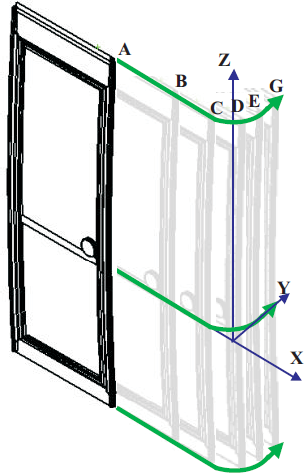
\includegraphics[width=.35\linewidth]{983_00}%
\end{center}


Pour des raisons de simplicité, l’étude du modèle sera faite uniquement pendant
la phase de verrouillage. Bien que pendant cette phase, les déplacements de la
porte se fassent suivant les deux directions $\vect{x}$ et $\vect{y}$, dans un souci d’obtenir des
modèles de comportement simples, on supposera, au regard du dimensionnement
adopté, que le déplacement suivant $\vect{x}$ est négligeable dans la phase considérée.
La validation de cette hypothèse ne rentrera pas dans le cadre de cette
étude.


\subsubsection*{Notations}
\begin{itemize}
\item $I_S$ : moment d’inertie du stator du motoréducteur suivant l’axe $\axe{I}{z_1}$.
\item $I_R$ : moment d’inertie du rotor suivant $\axe{I}{z_1}$.
\item $M_y$ : ensemble des masses en déplacement suivant la direction $\vect{y}$.
\item $N$ : rapport, supposé constant, entre les vitesses angulaires du rotor et du stator $\Omega_{4/1}=N\Omega_{1/0}$. On utilisera par la suite les notations suivantes $\Omega_S=\Omega_{1/0}$ et $\Omega_m = \Omega_{4/1}$.
\item $N_1\left(\theta_m\right)$ : rapport entre la vitesse d’un vantail par rapport à la voiture suivant $\vect{y}$ et la vitesse du stator $\Omega_S$, soit $V_y=N_1\left(\theta_m\right)\Omega_S$ où $\theta_m$ désigne l’angle de rotation
du rotor par rapport au stator.
\item $C_m$ : couple moteur.
\item $\vect{F}$ : force exercée par le(s) passager(s) suivant l’axe $\vect{y}$ avec $\vect{F}=F(t)\vect{y} $  (force due
par exemple, à une « pression » exercée par les passagers en cas de surcharge).
\end{itemize}

On suppose que pendant les opérations d’ouverture/fermeture la voiture est
immobile par rapport au sol dont tout repère $\rep{g}$ qui lui est attaché est considéré
comme galiléen.

%\subparagraph{}
%\textit{Montrer que l’évolution de la vitesse de rotation du stator est
%régie par l’équation différentielle suivante :
%$I_{eq}\left( \theta_m\right)\dot{\Omega}_S  =AC_m-B\left( \theta_m\right)\Omega_m^2-C\left( \theta_m\right)F$.
%Exprimer $I_{eq}\left( \theta_m \right)$, $A$, $B\left(\theta_m\right)$ et $C\left(\theta_m\right)$ en fonction de $I_S$, $I_R$, $M_y$, $N$, $N_1\left(\theta_m\right)$ et $N'_1\left(\theta_m\right)$ où $N'_1\left(\theta_m\right) = \dfrac{\partial N_1\left(\theta_m\right)}{\partial \theta_m}$. On suppose que toutes les liaisons sont parfaites
%et que l’action de la pesanteur est négligée pour toutes les pièces.}
%\ifprof
%\begin{corrige}
%
%\end{corrige}
%\else
%\fi

%L’équation différentielle suivante :
%$I_{eq}\left( \theta_m\right)\dot{\Omega}_S  =AC_m-B\left( \theta_m\right)\Omega_m^2-C\left( \theta_m\right)F$.

L’objectif de cette question est de définir un modèle de comportement
linéaire permettant de synthétiser un régulateur pour la chaîne d’asservissement
du moteur. On note :
\begin{itemize}
\item $\Omega_{m0}$ la vitesse de rotation du moteur, supposée constante;
\item $\theta_{m0}(t)$ la position angulaire de l’arbre moteur.
\end{itemize}
La linéarisation sera effectuée en utilisant l’équation différentielle obtenue à la
question précédente et les équations de comportement d’une
machine à courant continu.

L’inductance d’induit sera négligée, soit $L=0$.
L’ensemble des relations nécessaire à la mise en place du modèle est :
\begin{itemize}
 \item $I_{\text{eq}}\left( \theta_m\right)\dot{\Omega}_S = AC_m-B\left( \theta_m\right)\Omega_m^2-C\left( \theta_m\right)F$.
 \item $u(t)=Ri_m(t)+K_e\Omega_m(t)$, 
 \item $C_m(t)=K_ci_m(t)$.
\end{itemize}

%On a de plus  $I_{\text{eq}}(m)=I_S+I_R\left(N+1\right)^2+M_y\left(N_1\left(\theta_m\right)\right)^2$, $A=N$, $B=\dfrac{M_y N_1\left( \theta_m\right)N'_1\left( \theta_m\right)}{N}$ et $C\left( \theta_m\right)=-N_1\left( \theta_m\right)$.

\subparagraph{}
\textit{Préciser les relations liant :
\begin{itemize}
\item le couple moteur $C_{m0}\left(\theta_{m0}\right)$, la vitesse de rotation $\Omega_{m0}$ et la force due à la
poussée des passagers $F(t)=F_0$ supposée constante en fonction de $A$, $B$ et $C$;
\item le couple moteur $C_{m0}\left(\theta_{m0}\right)$ à la tension $U_{0}\left(\theta_{m0}\right)$ aux bornes de l’induit en fonction de la vitesse du moteur $\Omega_{m0}$ et des paramètres du moteur.
\end{itemize}}
\ifprof
\begin{corrige}
\end{corrige}
\else
\fi

Soient les variations $c_{m1}(t)$, $\Omega_1(t)$, $f_1(t)$ et $u_1(t)$ autour du régime d’équilibre
déterminé à la question précédente :
$C_m(t)=C_{m0}\left( \theta_{m0}\right)+c_{m1}(t)$, $\Omega_m(t)=\Omega_{m0}+\Omega_1(t)$, 
$F(t)=F_0+f_1(t)$ et $u(t)=U_0\left(\theta_{m0} \right)+u_1(t)$.



\subparagraph{}
\textit{Déterminer une équation différentielle, à paramètres variant dans le temps,
décrivant l’évolution de la variation de vitesse du moteur $\Omega_1$ autour du point de
fonctionnement décrit par $\left( \theta_{m0}, \Omega_{m0}, F_0, U_0\right)$. Exprimer cette équation sous la
forme : $\tau\left(\theta_{m0}\right)\dot{\Omega}_1(t)+{\Omega}_1(t)=K\left( \theta_{m0} \right)u_1(t)-D\left( \theta_{m0} \right)f_1(t)$.
Exprimer les paramètres $\tau$, $K$ et $D$ en fonction de $I_{eq}$, $A$, $B$, $C$, $N$, $\Omega_{m0}$ et les
paramètres du moteur.}
\ifprof
\begin{corrige}
\end{corrige}
\else
\fi


La position $\theta_{m0}$ de l’arbre moteur variant dans le temps, les coefficients de
l’équation différentielle précédente peuvent être modélisés comme des paramètres incertains qu’il est possible d’écrire sous la forme d’une partie connue constante
et d’une variation, soit :
$\tau\left(\theta_{m0}\right)=\tau_0\left(1+\delta t \right)$, $K\left(\theta_{m0}\right)=K_0\left(1+\delta K \right)$
et $D\left(\theta_{m0}\right)=D_0\left(1+\delta d \right)$.


\subparagraph{}
\textit{En supposant en première approximation que les variations sont nulles, déterminer
les fonctions de transfert $\dfrac{\Omega_1(p)}{U_1(p)}$ et $\dfrac{\Omega_1(p)}{F_1(p)}$ en les écrivant
sous une forme canonique en fonction de $\tau_0$, $K_0$ et $D_0$.}
\ifprof
\begin{corrige}
\end{corrige}
\else
\fi

 \begin{rem}L’analyse du comportement dû aux variations des paramètres ne
fait pas partie de cette étude.
\end{rem}



\subparagraph{}
\textit{Montrer que la fonction de transfert $\dfrac{\Omega_1(p)}{U_1(p)}$ peut être approchée sous
la forme $\dfrac{K_1}{p}$. Préciser le domaine de validité et exprimer $K_1$ en fonction de $\tau_0$
et $K_0$.}
\ifprof
\begin{corrige}
\end{corrige}
\else
\fi


\begin{enumerate}
%\item.
\item $AC_{m0}-B\left( \theta_{m0}\right) \Omega_{m0}^2-C\left( \theta_{m0}\right)F_0 = 0 $ et $C_{m0}(t)=\dfrac{K_C}{R}\left(U_0-K_e\Omega_{m0}\right)$
\item $\dfrac{RI_{eq}\left( \theta_m\right)}{N\left( AK_cK_e+2RB\left( \theta_m\right)\Omega_{m0}\right)} \dot{\Omega}_1+\Omega_1 $

 $= 
\dfrac{AK_c}{ AK_cK_e+2RB\left( \theta_m\right)\Omega_{m0}} u_1
- \dfrac{RC\left( \theta_m\right)}{ AK_cK_e+2RB\left( \theta_m\right)\Omega_{m0}} f_1$
\item $\dfrac{\Omega_1(p)}{U_1(p)}=\dfrac{K_0}{1+\tau_0 p}$ et $\dfrac{\Omega_1(p)}{F_1(p)}=-\dfrac{D_0}{1+\tau_0 p}$.
\item ...
\end{enumerate}
